% begin module trig-functions-graphs
\begin{frame}
\frametitle{Graphs of the Trigonometric Functions}
\begin{tabular}{cc}
\begin{tabular}{c}
\psset{xunit=0.6cm,yunit=0.6cm}
\begin{pspicture}(-5,-1.4)(10,1.4)
\tiny
\psaxes[labels=none, Dx=1.570796327, Dy=1] {<->}(0,0)(-4,-1.4)(10,1.4)
\psplot[linecolor=red, plotpoints=1000]{-4}{10}{x 57.295779513 mul sin}

\rput[t](-3.14, -0.3){$-\pi$}
\rput[t](-1.57, -0.3){$-\frac{\pi}{2}$}
\rput[t](1.57, -0.3){$\frac{\pi}{2}$}
\rput[t](3.14, -0.3){$\pi$}
\rput[t](4.71, -0.3){$\frac{3\pi}{2}$}
\rput[t](6.28, -0.3){$2\pi$}
\rput[t](7.85, -0.3){$\frac{5\pi}{2}$}
\rput[t](9.42, -0.3){$3\pi$}
\rput[bl](0.2,1){\tiny $1$}
\end{pspicture}
%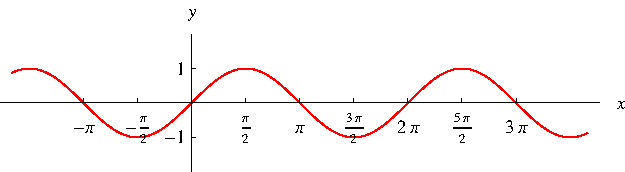
\includegraphics[width=8cm]{trigonometry/pictures/app-d-sin.pdf}%

\end{tabular}
& $y = \sin x$\\
\begin{tabular}{c}
\psset{xunit=0.6cm,yunit=0.6cm}
\begin{pspicture}(-5,-1.4)(10,1.4)
\tiny
\psaxes[labels=none, Dx=1.570796327, Dy=1] {<->}(0,0)(-4,-1.4)(10,1.4)
\psplot[linecolor=red, plotpoints=1000]{-4}{10}{x 57.295779513 mul cos}

\rput[t](-3.14, -0.3){$-\pi$}
\rput[t](-1.57, -0.3){$-\frac{\pi}{2}$}
\rput[t](1.57, -0.3){$\frac{\pi}{2}$}
\rput[t](3.14, -0.3){$\pi$}
\rput[t](4.71, -0.3){$\frac{3\pi}{2}$}
\rput[t](6.28, -0.3){$2\pi$}
\rput[t](7.85, -0.3){$\frac{5\pi}{2}$}
\rput[t](9.42, -0.3){$3\pi$}
\rput[bl](0.2,1){\tiny $1$}
\end{pspicture}
%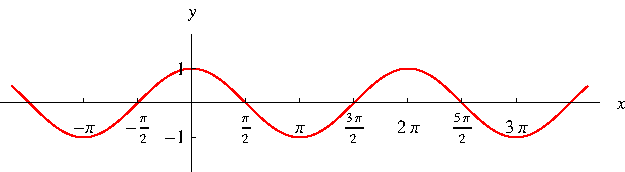
\includegraphics[width=8cm]{trigonometry/pictures/app-d-cos.pdf}%
\end{tabular}
& $y = \cos x$
\end{tabular}
\begin{itemize}
\item<2->  $\sin x$ has zeroes at $n\pi$ for all integers $n$.
\item<3->  $\cos x$ has zeroes at $\pi /2 + n\pi$ for all integers $n$.
\item<4->  $-1 \leq \sin x \leq 1$. 
\item<5->  $-1 \leq \cos x \leq 1$. 
\end{itemize}
\end{frame}





% end module trig-functions-graphs
